\documentclass{beamer}
\usetheme{Boadilla}
\usecolortheme{seahorse}
\usepackage{listings}
\lstset{
%language=C,
frame=single, 
breaklines=true,
columns=fullflexible
}
\usepackage{subcaption}
\usepackage{url}
\usepackage{tikz}
\usepackage{graphicx}
\usepackage{tkz-euclide} % loads  TikZ and tkz-base
%\usetkzobj{all}
\usetikzlibrary{calc,math}
\usepackage{float}
\newcommand\norm[1]{\left\lVert#1\right\rVert}
\renewcommand{\vec}[1]{\mathbf{#1}}
\newcommand{\R}{\mathbb{R}}
\newcommand{\C}{\mathbb{C}}
\providecommand{\brak}[1]{\ensuremath{\left(#1\right)}}
\providecommand{\abs}[1]{\vert#1\vert}
\providecommand{\fourier}{\overset{\mathcal{F}}{ \rightleftharpoons}}
\providecommand{\pr}[1]{\ensuremath{\Pr\left(#1\right)}}
\providecommand{\sbrak}[1]{\ensuremath{{}\left[#1\right]}}
\usepackage[export]{adjustbox}
\usepackage[utf8]{inputenc}
\usepackage{amsmath}

\title{More Probability Estimators for CABAC in Versatile Video Coding}
\author{Varenya Upadhyaya}
\institute{IITH}
\date{\today}
\begin{document}
\begin{frame}
\titlepage
\end{frame}
\begin{frame}{About the paper}
\begin{block}{Authors}
    \begin{enumerate}[]
        \item Sio-Kei Im
        \item Ka-Hou Chan
    \end{enumerate}
\end{block}

\begin{block}{Institute}
\begin{enumerate}[]
    \item Macao Polytechnic Institute %\\
    % Macao, China
\end{enumerate}
\end{block}

\begin{block}{Time of Publishing}
\begin{enumerate}[]
    \item October, 2020
\end{enumerate} 
\end{block}
\end{frame}
\section{Terms and Definitions}
\begin{frame}{Video Coding Format}
The compression of a digital video is usually done using a video coding format: 
\begin{enumerate}[]
    \item A V.C.F. is a content representation format for storage or transmission of digital video content.
    \item It uses a video compression algorithm based on Discrete Cosine Transforms and Motion Compensation.%(Motion compensation is an algorithmic technique used to predict a frame in a video, given the previous and/or future frames by accounting for motion of the camera and/or objects in the video)
\end{enumerate}
Examples: 
\begin{enumerate}[]
    \item AVC[2003]: Advanced Video Coding (Blu-ray, HDTV, Streaming etc.)
    \item HEVC[2013]: High Efficiency Video Coding (UHD Blu-ray, UHD streaming, macOS High Sierra)
    \item VVC[2020]: Versatile Video Coding
\end{enumerate}
\end{frame}
\begin{frame}{Types of Video Compression}
There are three main subdivisions in video coding formats:
\begin{enumerate}
    \item Lossy: Uses partial data and inexact approximations to represent content (mainly found in consumer video).
    \item Lossless: Allows the original data to be perfectly reconstructed using the compressed data.
    \item Uncompressed: Digital Video that has never been compressed (Clean HDMI, video cameras, video monitors etc.).
\end{enumerate}
    
\end{frame}

\begin{frame}{Versatile Video Coding}
\begin{block}{Introduction}
\begin{enumerate}[]
  \item Versatile Video Coding (VVC) is a video compression standard finalized on 6 July 2020.
  \item It is the successor to HEVC. 
  \item The aim is to make 4K broadcast and streaming commercially viable.
\end{enumerate}
\end{block}
\begin{block}{Concept for VVC} 
\begin{enumerate}[]
    \item 30–50\% better compression rate for the same perceptual quality
    \item  Should support lossless and subjectively lossless compression
    \item Should support resolutions from 4K to 16K as well as 360° videos
\end{enumerate}
\end{block}

\end{frame}
\section{CABAC}
\begin{frame}{CABAC}
\begin{enumerate}[]
    \item Contex-based Adaptive Binary Arithmetic Coding is and entropy coding system used in AVC, HEVC and VVC.\\
    \item It performs integer bit operations on all floating point type calculations\\
    \item CABAC has multiple probability modes for different contexts. 
    \item It first converts all non-binary symbols to binary then, for each bit, the coder selects which probability model to use, and then uses information from nearby elements to optimize the probability estimate. 
    \item Arithmetic coding is finally applied to compress the data.
\end{enumerate}

\end{frame}

\begin{frame}{CABAC in HEVC}
\begin{enumerate}[]
\item There are 64 values(finite states) used to represent an accurate estimation.
\item Each value has assigned one of 64 representative values dividing the range of $[0.01875,0.5]$
\end{enumerate}   
The update in probabilities in the context model is based on: 
\begin{align}
    P(t+1)=\label{prob_1}
    \begin{cases}
    \alpha\cdot P(t)&\text{MPS}\\
    1-\alpha\cdot(1-P(t))&\text{LPS}
    \end{cases}
\end{align}
where, MPS and LPS are the Most Probable Symbols and Least Probable Symbols respectively;
$P(t+1)$ is the probability of receiving LPS.
\end{frame}
\begin{frame}{Determination of \alpha }
     $\alpha$ is the adaptation rate and has a constant value
\begin{align}
    \alpha = \sqrt[63]{0.01875/0.5} \approx 0.949
\end{align}
\begin{enumerate}
    \item Probability estimation in CABAC is based on a table-driven estimator using a finite-state machine (FSM) approach
    \item The method for designing the FSM transition rules was borrowed from HOWARD and VITTER using a model of "exponential aging" which gives rise to the state transition relation \eqref{prob_1}\\
\end{enumerate}
    According to \eqref{prob_1}, the scaling factor a can be determined by 
    \begin{align}
        P_{min} = 0.5 \alpha^{N-1}
    \end{align}
    with the choice of $P_{min} = 0.01875$ and $N = 64$
    \begin{align}
    \implies\alpha = \sqrt[63]{0.01875/0.5} 
    \end{align}

\end{frame}
\begin{frame}{CABAC in VVC}
\begin{enumerate}[]
    \item VVC introduces a new concept that this adaptation rate becomes dynamic during the process of arithmetic coding.
    \item The context model updates according to the value of the currently encoded symbol.
    \item The adaptation rate is controlled by two context models in parallel with parameters $r_0$ and $r_1$ :
\end{enumerate}

\begin{align}
    P_i(t+1) =\label{vvc_1}
    \begin{cases}
        \brak{1-\frac{1}{2^{r_i}}}\cdot P_i(t)&\text{MPS}\\\\
        1-\brak{1-\frac{1}{2^{r_i}}}\cdot(1-P_i(t))&\text{LPS}
    \end{cases}
\end{align}
where $i \in \{0,1\}$ and $r_i$ is exponentially weighted related to the coding mode.\\
The updated probability will be the average of $P_i(t+1)$ 
\end{frame}
\begin{frame}{CABAC in VVC}
\begin{enumerate}
\item The purpose of using two parameters is to achieve an optimal update speed.
\item By using different parameters, the shift value can be adapted when the probability changes in the context of obtaining the best effect between the drops rate balances.
\item Instead of the lookup table, VVC uses a linearly quantized probability representation and arithmetic operations to update the probability, which allows adaptation to occur for more situations without the restriction of 64 states in HEVC.
\end{enumerate}
\end{frame}
\section{Parameters}
\begin{frame}{More Parameter Probability Estimation}
In VVC CABAC, there are two context models and their quantization estimator requires 15bits for probability presentation and then 10 and 14 bits for two hypothetical probability estimates:
\begin{figure}[h]
    \centering
    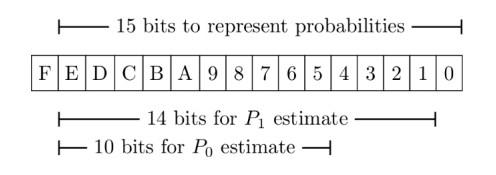
\includegraphics{vvc_param.jpg}
    \caption{15 bits to represent probabilities , 10 and 14 for $P_0$ and $P_1$ resp.}
    \label{fig:original_vvc}
\end{figure}

\end{frame}

\begin{frame}{Continued}
    For each update of $P_0$ and $P_1$, the high 10 and 14 bits are kept for probability estimation while the low 1 and 5 bits are discarded to 0.
\begin{align}
    0<P_0\leq P_1< 2^{15}
\end{align}
While the drop rate $\alpha$ must satisfy
\begin{align}
        \brak{1-\frac{1}{2^0}}&<\alpha<\brak{1-\frac{1}{2^{15}}}
\end{align}
Further, since all division is done using bit shift operations, the number of shifts cannot exceed the defined 15 bits. 
\begin{align}
    r_i&\in \{1,2\cdots 14\}\\
    r_0&<r_1
\end{align}
\end{frame}
\begin{frame}{Proposed update}
Under the new system, the bits are distributed as follows:
\begin{figure}
    \centering
    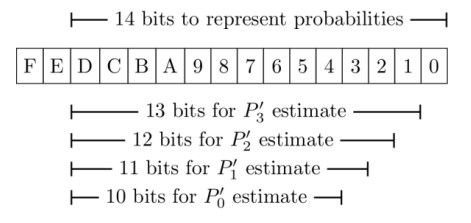
\includegraphics{vvc_param_prop.jpg}
    \caption{Proposed set of parameters}
    \label{fig:proposed_vvc}
\end{figure}
\begin{enumerate}[]
    \item 14 bits to handle probability estimation.
    \item highest bit to represent MPS symbol
    \item second highest to prevent overflow.
\end{enumerate}
\end{frame}
\begin{frame}{Continued}
Corresponding to the bit distribution, the following inferences can be made:
    \begin{align}
        0\leq {P'}_0\leq {P'}_1\leq {P'}_2\leq {P'}_3<2^{14}\\
        \brak{1-\frac{1}{2^0}}<\alpha '<\brak{1-\frac{1}{2^{14}}}
    \end{align}
    Range of the parameters: 
    \begin{align}
        r'_i \in \{1,2,\cdots 13\}\\
        r'_0<r'_1<r'_2<r'_3
    \end{align}
\end{frame}
\begin{frame}{Drop rate consideration}
    In the original VVC model, the parameters were preset for different coding modes (so that the drop rates cannot be adjusted at will); the same preset parameters are used in the proposed model: 
    \begin{align}
        r'_0 &= r_0\label{param_1}\\
        r'_1 &= \frac{3}{4}r_0 + \frac{1}{4}r_1\\
        r'_2 &= \frac{1}{4}r_0 + \frac{3}{4}r_1\\
        r'_3 &= r_1\label{param_3}
    \end{align}
    \eqref{param_1} and \eqref{param_3} are first used to determine the boundaries of the parameters and the other parameters are calculated from there using linear interpolation.\\

\end{frame}
\begin{frame}{Continued}
\begin{enumerate}[]
    \item The proposed model can replace $P_i(t+1)$ in \eqref{vvc_1} with $P'_i(t+1)$\\
    \item Based on the drop rate $r'_i$, four estimators can be determined as follows:
    \begin{align}
        P'_i(t+1)=
        \begin{cases}
            \brak{1-\frac{1}{2^{r'_i}}}\cdot P'_i(t) & \text{MPS}\\\\
            \frac{1}{2^{r'_i}} + \brak{1-\frac{1}{2^{r'_i}}}\cdot P'_i(t)&\text{LPS}
        \end{cases}
    \end{align}
    \end{enumerate}
\end{frame}
\begin{frame}{MPS Determination}
    % \begin{enumerate}
    According to the definition of CABAC, $P(t+1)$ is the probability of receiving LPS. 
    This implies $P(t+1)<0.5$\\
    From \eqref{prob_1}, we get the following conditions:
    \begin{align}
        P(t+1)&<P(t) \text{ if MPS is received}\\
        P(t+1)&>P(t) \text{ otherwise}
    \end{align}
    When $P(t+1)>0.5$, (caused by receiving the LPS continuously) the symbols for MPS and LPS will be swapped.
    This is used to determine the MPS and it can be applied to the next gen as follows:
    \begin{align}
        P'(t+1) = \frac{1}{4}\sum_{i=0}^{3} P_i'(t+1)>0.5\\
        \implies \sum_{i=0}^{3} P_i'(t+1)>2\label{dec_val}
    \end{align}
    % \end{enumerate}
\end{frame}
\begin{frame}{Continued}
\begin{enumerate}[]
\item The range of probabilities $[0.0, 1.0]$ will be scaled to $[2^0, 2^{14}]$ using integers. 
\item Thus the decision value in \eqref{dec_val} will be scaled to $2\times2^{14}=2^{15}$; at the highest index (F) in Fig. \ref{fig:proposed_vvc} 
\item This is why it was mentioned that the highest bit is reserved for MPS representation.
\end{enumerate}    
\end{frame}
\section{Process}
\begin{frame}{Updating process}
    \begin{figure}
        \centering
        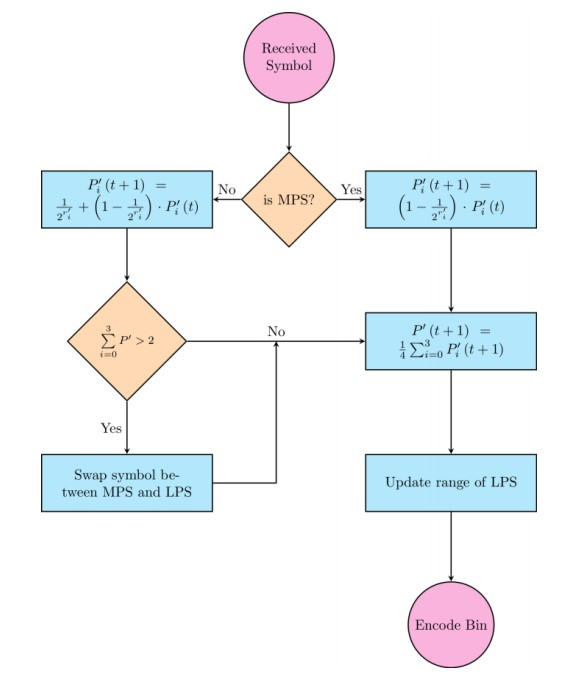
\includegraphics[width=55mm]{flowchart.jpg}
        \caption{Flowchart for symbol processing and probability estimation}
        \label{fig:flow}
    \end{figure}
\end{frame}
\begin{frame}{Continued}
    Essence of the flowchart:
    \begin{enumerate}
        \item Check if the received symbol is MPS.
        \item if yes, calculate $P'_i(t+1)$ using \eqref{vvc_1} for MPS.
        \item then calculate $P'(t+1)$ by averaging $P'_i(t+1)$
        \item accordingly update the range of LPS.
        \item if no, calculate $P'_i(t+1)$ using \eqref{vvc_1} for LPS.
        \item check if the sum is greater than $2$ (as per \eqref{dec_val})
        \item if yes, swap MPS and LPS, else simply calculate $P'(t+1)$ and update the range of LPS accordingly.
    \end{enumerate}
\end{frame}

\begin{frame}{Continued}
\begin{enumerate}[]
        \item In HEVC, this part was carried out using a lookup table,  so the probabilities can only provide a finite set of values; which is inefficient for floating point calculations. 
        \item Linear quantization is useful as the number of digits in Fig. \ref{fig:proposed_vvc} may increase at any time (for which a lookup table would not work). 
        \item The quantization proposed by VVC requires 10 and 14 bits to store probability estimates of the hypotheses while the method proposed in the paper uses 11-13 bits to achieve better compression efficiency. 
\end{enumerate}
\end{frame}
\section{Experiments}
\begin{frame}{Experimental results}
    \begin{figure}
        \centering
        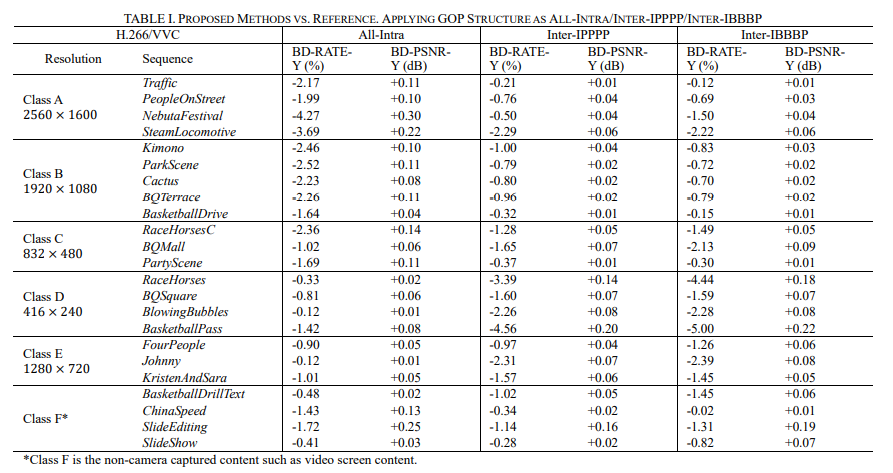
\includegraphics[width=120mm]{exp_table.png}
        % \caption{Caption}
        \label{fig:my_label}
    \end{figure}
\end{frame}
\begin{frame}{Continued}
    \begin{figure}
        \centering
        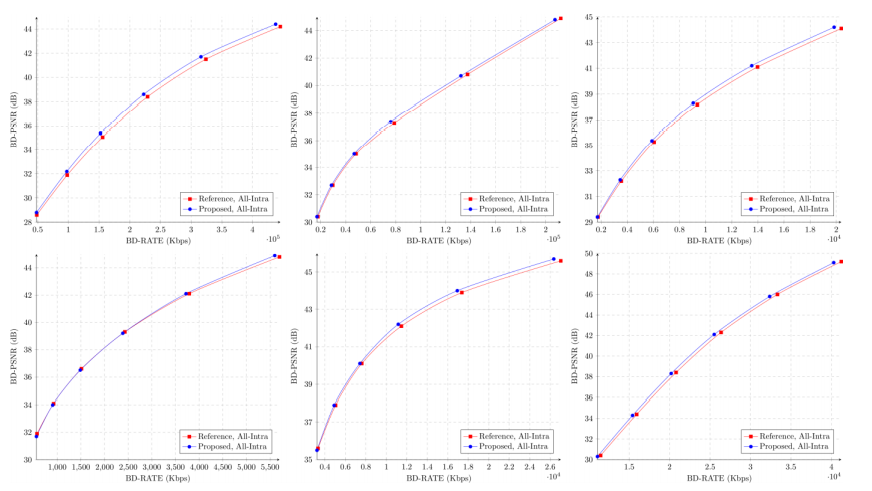
\includegraphics[width=120mm]{exp_graphs.png}
        \caption{Graphs for the reference and proposed observations}
        \label{fig:exp_g}
    \end{figure}
\end{frame}
\section{Conclusion}
\begin{frame}{In conclusion...}
    \begin{enumerate}
        \item Different drop rates are used to achieve flexibility in order to make the estimators usable for sources with different statistical information
        \item A major design aspect is the compatibility of having more drop rate decisions and making use of linear quantization instead of finite states in CABAC.
        \item This is achieved by using a more compact representation of the probability state, and a multiplication free operation is achieved through a series of bit operations
        \item Experiments show that more estimator representations used for encoding lead to better optimization mode decisions without incurring significant complexity overhead. 
        \item The improvement shows that gain is provided in the encoding, and the proposed method can be used in the next generation VVC standard
    \end{enumerate}
\end{frame}

\end{document}